\documentclass[a4paper]{article}
\usepackage{german}
\usepackage[utf8]{inputenc}

\usepackage{pgfplots}
\usepackage{pgfplots.assert}

\usetikzlibrary{intersections}
\usetikzlibrary{pgfplots.decorations.softclip}
\usepgflibrary{fillbetween}

\begin{document}
\thispagestyle{empty}
\parindent=0pt
\parskip10pt

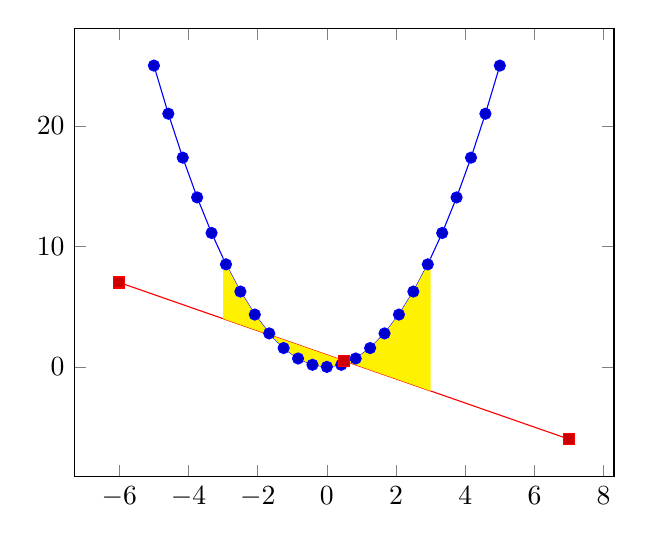
\begin{tikzpicture}
	\begin{axis}
	\addplot+[name path global=A] {x^2};

	\addplot+[name path global=B,domain=-6:7,samples=3] {1-x};

	\path[name path=clip] (axis cs:-3,-5) rectangle (axis cs:3,20);

	\fill[yellow]
		\pgfextra
		\expandafter\let\expandafter\clipper\csname tikz@intersect@path@name@clip\endcsname
		\pgffillbetweensetsoftclippathfirst{\clipper}%
		\pgffillbetweensetsoftclippathsecond{\clipper}%

		\expandafter\let\expandafter\A\csname tikz@intersect@path@name@A\endcsname
		\expandafter\let\expandafter\B\csname tikz@intersect@path@name@B\endcsname
		\pgfpathfillbetween{\A}{\B}
		\endpgfextra
	;% 
	\end{axis}
\end{tikzpicture}



\end{document}

